\documentclass{beamer}
\mode<presentation>
\usepackage{amsmath}
\usepackage{amssymb}
%\usepackage{advdate}
\usepackage{graphicx}
\usepackage{adjustbox}
\usepackage{subcaption}
\usepackage{enumitem}
\usepackage{multicol}
\usepackage{mathtools}
\usepackage{listings}
\usepackage{url}
\def\UrlBreaks{\do\/\do-}
\usetheme{Boadilla}
\usecolortheme{lily}
\setbeamertemplate{footline}
{
  \leavevmode%
  \hbox{%
  \begin{beamercolorbox}[wd=\paperwidth,ht=2.25ex,dp=1ex,right]{author in head/foot}%
    \insertframenumber{} / \inserttotalframenumber\hspace*{2ex} 
  \end{beamercolorbox}}%
  \vskip0pt%
}
\setbeamertemplate{navigation symbols}{}

\providecommand{\nCr}[2]{\,^{#1}C_{#2}} % nCr
\providecommand{\nPr}[2]{\,^{#1}P_{#2}} % nPr
\providecommand{\mbf}{\mathbf}
\providecommand{\pr}[1]{\ensuremath{\Pr\left(#1\right)}}
\providecommand{\qfunc}[1]{\ensuremath{Q\left(#1\right)}}
\providecommand{\sbrak}[1]{\ensuremath{{}\left[#1\right]}}
\providecommand{\lsbrak}[1]{\ensuremath{{}\left[#1\right.}}
\providecommand{\rsbrak}[1]{\ensuremath{{}\left.#1\right]}}
\providecommand{\brak}[1]{\ensuremath{\left(#1\right)}}
\providecommand{\lbrak}[1]{\ensuremath{\left(#1\right.}}
\providecommand{\rbrak}[1]{\ensuremath{\left.#1\right)}}
\providecommand{\cbrak}[1]{\ensuremath{\left\{#1\right\}}}
\providecommand{\lcbrak}[1]{\ensuremath{\left\{#1\right.}}
\providecommand{\rcbrak}[1]{\ensuremath{\left.#1\right\}}}
\theoremstyle{remark}
\newtheorem{rem}{Remark}
\newcommand{\sgn}{\mathop{\mathrm{sgn}}}
\providecommand{\abs}[1]{$\left\vert#1\right\vert$}
\providecommand{\res}[1]{\Res\displaylimits_{#1}} 
\providecommand{\norm}[1]{\lVert#1\rVert}
\providecommand{\mtx}[1]{\mathbf{#1}}
\providecommand{\mean}[1]{E$\left[ #1 \right]$}
\providecommand{\fourier}{\overset{\mathcal{F}}{ \rightleftharpoons}}
%\providecommand{\hilbert}{\overset{\mathcal{H}}{ \rightleftharpoons}}
\providecommand{\system}[1]{\overset{\mathcal{#1}}{ \longleftrightarrow}}
%\providecommand{\system}{\overset{\mathcal{H}}{ \longleftrightarrow}}
	%\newcommand{\solution}[2]{\textbf{Solution:}{#1}}
%\newcommand{\solution}{\noindent \textbf{Solution: }}
\providecommand{\dec}[2]{\ensuremath{\overset{#1}{\underset{#2}{\gtrless}}}}
\newcommand{\myvec}[1]{\ensuremath{\begin{pmatrix}#1\end{pmatrix}}}
\let\vec\mathbf

\lstset{
%language=C,
frame=single, 
breaklines=true,
columns=fullflexible
}

\numberwithin{equation}{section}

\title{5.3.18}
\author{AI25BTECH11024 - Pratyush Panda}
\begin{document}
\maketitle

\begin{frame}
\textbf{Question: } \\
Using matrix method, solve the following system of equations
\begin{align}
2x - 3y + 5z = 13 \\
3x + 2y - 4z = -2 \\
x + y - 2z = -2
\end{align}
\end{frame}

\begin{frame}
\textbf{Solution: } \\
The given system of equations can be written as;
\begin{align}
\Vec{A}\Vec{X}=\Vec{B} \hspace{0.5cm} where, \, \Vec{A}=\myvec{2 & -3 & 5 \\ 3 & 2 & -4 \\ 1 & 1 & -2}, \, \Vec{B}=\myvec{13 \\ -2 \\ -2} \, and \, \Vec{X}=\myvec{x \\ y \\ z}
\end{align}\

Now, since $\Vec{A}$ is not a singular matrix we can pre-multiply both sides with $\Vec{A}^{-1}$\\
From that we get;
\begin{align}
\Vec{X}=\Vec{A}^{-1}\Vec{B}
\end{align}
\end{frame}

\begin{frame}
On solving for $\Vec{A}^{-1}$ we get $\Vec{A}^{-1}=\myvec{0 & 1 & -2 \\ -2 & 9 & -23 \\ -1 & 5 & -13}$ \\

Thus,
\begin{align}
\Vec{X}=\Vec{A}^{-1}\Vec{B}=\myvec{0 & 1 & -2 \\ -2 & 9 & -23 \\ -1 & 5 & -13}\myvec{13 \\ -2 \\ -2} \\
or, \, \Vec{X}=\myvec{2 \\ 2 \\ 3}
\end{align}

Thus, the solution set is $\brak{x,y,z}=\brak{2,2,3}$.
\end{frame}

\begin{frame}
\begin{figure}[H]
\centering
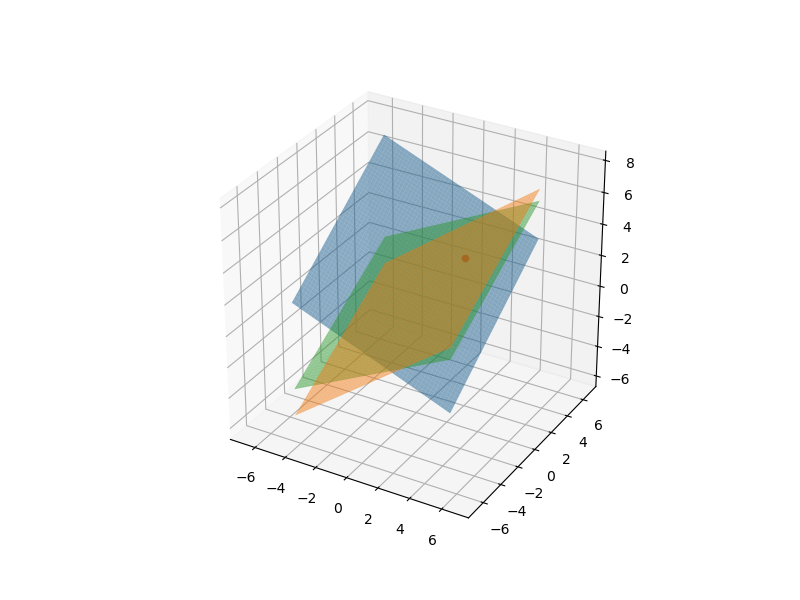
\includegraphics[width=0.6\columnwidth]{figs/img.png}
\caption*{}
\end{figure}
\end{frame}

\end{document}
